% Institute of Computer Science thesis template
% authors: Sven Laur, Liina Kamm
% last change Tõnu Tamme 03.05.2019
%--
% Compilation instructions:
% 1. Choose main language on line 55-56 (English or Estonian)
% 2. Compile 1-3 times to get refences right
% pdflatex bachelors-thesis-template
% bibtex bachelors-thesis-template
%--
% Please use references like this:
% <text> <non-breaking-space> <cite/ref-command> <punctuation>
% This is an example~\cite{example}.

\documentclass[12pt]{article}

% A package for setting layout and margins for your thesis 
\usepackage[a4paper]{geometry}

\setlength{\parindent}{0em}
\setlength{\parskip}{1em}
\usepackage{setspace}
\onehalfspace

\usepackage[utf8]{inputenc} %standard encoding since 2018 (can be commented out?)
\usepackage[T1]{fontenc} %Absolutely critical for *hyphenation* of words with non-ASCII letters.

% Typeset text in Times Roman instead of Computer Modern (EC)
\usepackage{times}

% Suggested packages:
\usepackage{microtype}  %towards typographic perfection...
\usepackage{inconsolata} %nicer font for code listings. (Use \ttfamily for lstinline bastype)

\usepackage[english, estonian]{babel} %the thesis is in Estonian

% Change Babel document elements 
\addto\captionsestonian{%
    \renewcommand{\refname}{Viidatud kirjandus}%
    \renewcommand{\appendixname}{Lisad}%
}


% If you have problems with Estonian keywords in the bibliography
%\usepackage{biblatex}
%\usepackage[backend=biber]{biblatex}
%\usepackage[style=alphabetic]{biblatex}
%% plain --> \usepackage[style=numeric]{biblatex}
%% abbrv --> \usepackage[style=numeric,firstinits=true]{biblatex}
%% unsrt --> \usepackage[style=numeric,sorting=none]{biblatex}
%% alpha --> \usepackage[style=alphabetic]{biblatex}
%\DefineBibliographyStrings{estonian}{and={ja}}
%\addbibresource{bachelor-thesis.bib}


% General packages for math in general, theorems and symbols 
% Read ftp://ftp.ams.org/ams/doc/amsmath/short-math-guide.pdf for further information
\usepackage{amsmath}
\usepackage{amsthm}
\usepackage{amssymb}

% Print a dot instead of colon in table or figure captions
\usepackage[labelsep=period]{caption}

% Packages for building tables and tabulars 
\usepackage{array}
\usepackage{tabu}   % Wide lines in tables
\usepackage{xspace} % Non-eatable spaces in macros

% Including graphical images and setting the figure directory
\usepackage{graphicx}
%\graphicspath{{figures/}}

% Packages for getting clickable links in PDF file
%\usepackage{hyperref}
\usepackage[hidelinks]{hyperref} %hide red (blue,green) boxes around links
\usepackage[all]{hypcap}


% Packages for defining colourful text together with some colours
\usepackage{color}
\usepackage{xcolor}
%\definecolor{dkgreen}{rgb}{0,0.6,0}
%\definecolor{gray}{rgb}{0.5,0.5,0.5}
\definecolor{mauve}{rgb}{0.58,0,0.82}


% Standard package for drawing algorithms
% Since the thesis in article format we must define \chapter for
% the package algorithm2e (otherwise obscure errors occur) 
\let\chapter\section
\usepackage[ruled, vlined, linesnumbered]{algorithm2e}

% Fix a  set of keywords which you use inside algorithms
\SetKw{True}{true}
\SetKw{False}{false}
\SetKwData{typeInt}{Int}
\SetKwData{typeRat}{Rat}
\SetKwData{Defined}{Defined}
\SetKwFunction{parseStatement}{parseStatement}


% Nice todo notes
\usepackage{todonotes}

% comments and verbatim text (code)
\usepackage{verbatim}

% units
\usepackage{siunitx}
\sisetup{
    output-decimal-marker = {,},
    range-phrase={--},
    range-units=single
}
\DeclareSIUnit \belm {Bm}

% Nice Todo box
\newcommand{\TODO}{\todo[inline]}

\setlength{\abovecaptionskip}{10pt minus 6pt}

% non breaking dashes
\usepackage[shortcuts]{extdash}

%%% BEGIN DOCUMENT
\begin{document}

%===BEGIN TITLE PAGE
    \thispagestyle{empty}
    \begin{center}


        \large
        TARTU ÜLIKOOL\\
        Arvutiteaduse instituut\\
        Informaatika õppekava\\[2mm]


        \vspace*{\stretch{5}}
        \vspace{25mm}

        \Large Kert Tali

        \vspace{4mm}

        \huge LPWAN raadiovõrkude võrdlus ja kasutusjuhud Tartu näitel

%\vspace*{\stretch{7}}
        \vspace{20mm}

        \Large Bakalaureusetöö (9 EAP)

    \end{center}

    \vspace{2mm}

    \begin{flushright}
    {
        \setlength{\extrarowheight}{5pt}
        \begin{tabular}{r l}
            \sffamily Juhendaja: & \sffamily Alo Peets \\
        \end{tabular}
    }
    \end{flushright}

    \vspace*{\stretch{3}}
    \vspace{10mm}

    \vfill
    \centerline{Tartu 2020}

%===END TITLE PAGE

% If the thesis is printed on both sides of the page then 
% the second page must be must be empty. Comment this out
% if you print only to one side of the page comment this out
%\newpage
%\thispagestyle{empty}    
%\phantom{Text to fill the page}
% END OF EXTRA PAGE WITHOUT NUMBER


%===COMPULSORY INFO PAGE
    \newpage

%=== Info in English
    \newcommand\EngInfo{{%
        \selectlanguage{english}
        \noindent\textbf{\large Comparison and use cases of LPWAN networks in Tartu}
        \vspace*{1ex}

        \noindent\textbf{Abstract:}
        \TODO{Valmib lõpus}
        \noindent

        \vspace*{1ex}

        \noindent\textbf{Keywords:}\\
        IoT, LPWAN, LoRaWAN, Sigfox, NB-IoT, service comparison, use cases

        \vspace*{1ex}

        \noindent\textbf{CERCS:} T180 Telecommunication engineering; P170 Computer science, numerical analysis, systems, control

        \vspace*{1ex}
    }}%\newcommand\EngInfo


%=== Info in Estonian
    \newcommand\EstInfo{{%
        \selectlanguage{estonian}
        \noindent\textbf{\large LPWAN raadiovõrkude võrdlus ja kasutusjuhud Tartu näitel}
        \vspace*{1ex}

        \noindent\textbf{Lühikokkuvõte:}

%\noindent ...
        \TODO{Valmib lõpus}
%\TODO{One or two sentences providing a basic introduction to the field, comprehensible to a scientist in
%any discipline.}
%\TODO{Two to three sentences of
%more detailed background, comprehensible to scientists in related disciplines.}
%\TODO{One sentence clearly stating the general problem being addressed by this particular
%study.}
%\TODO{One sentence summarising the main result (with the words ``here we show´´ or their equivalent).}
%\TODO{Two or three sentences explaining what
%the main result reveals in direct
%comparison to what was thought to be the case previously, or how the main result adds to previous knowledge.}
%\TODO{One or two sentences to put the results into a more general context.}
%\TODO{Two or three sentences to provide a
%broader perspective, readily
%comprehensible to a scientist in any
%discipline, may be included in the first paragraph
%if the editor considers that the accessibility of
%the paper is significantly enhanced by their inclusion.}

        \vspace*{1ex}

        \noindent\textbf{Võtmesõnad:}\\
        IoT, LPWAN, LoRaWAN, Sigfox, NB-IoT, teenusvõrkude võrdlus, kasutusjuhud

        \vspace*{1ex}

        \noindent\textbf{CERCS:} T180 Telekommunikatsioonitehnoloogia; P170 Arvutiteadus, arvutusmeetodid, süsteemid, juhtimine (automaatjuhtimisteooria)

        \vspace*{1ex}
    }}%\newcommand\EstInfo


%=== Determine the order of languages on Info page
    {\EngInfo}{\EstInfo}


    \newpage
    \setlength{\parskip}{0em}
    \tableofcontents
    \setlength{\parskip}{1em}

% Remember to remove this from the final thesis version
%\newpage
%\listoftodos[Unsolved issues]
% END OF TODO PAGE 


    \newpage


    \section{Sissejuhatus}

%\TODO{What is it in simple terms (title)?}
%\TODO{Why should anyone care?}
%\TODO{What was my contribution?}
%\TODO{What you are doing in each section (a sentence or two per section)}

% TAUSTA LÜHIKIRJELDUS
    Suurenev vajadus nutistul põhinevate äri- ja mugavusrakenduste järele põhjustab ühest küljest võidujooksu uute IoT-lahenduste leiutamisele, mis on teisest küljest tagasi hoitud tehnoloogiliste ja füüsiliste piirangutega.
    Üks sellistest pudelikaeladest hõlmab seadmetevahelist suhtlust (\textit{Machine-to-Machine} ehk M2M), mille puhul tuleb arendajal valida olemasolevate sidetehnoloogiate seast oma rakendusele sobivaim.
    Traadita andmeside tehnoloogiate seas on populaarsust kogumas uus klass — LPWAN (\textit{Low Power Wide Area Network} ehk madala voolutarbe ja laia ulatusega võrk), mis on mõeldud rakendustele, mis eeldavad nii madalat voolutarvet kui laia leviala.
    Konkureerivad tehnoloogiad -- Sigfox, LoRa, NB-IoT, LTE-M, Ingenu ja Weightless reklaamivad seadmetele suurusjärgus kümneaastast aku eluiga ja kümnekilomeetrist levikaugust.

    Kuigi tehnoloogiad täidavad ühist nišši pakkuda laiahaardelist ja usaldusväärset ühenduvust ressursidest piiratud seadmetele, erinevad need oma võimekuse poolest märkimisväärselt.
    Uurimistöö eesmärk on hinnata Tartus kättesaadavate teenuste sobivust erinevatele asjade interneti kasutusjuhtudele, milleks võib olla näiteks tark arvesti kortermaja keldris või turvasüsteem maakodule.
    Selline ülevaade on väärtuslik lähtekoht väiksematele teenusepakkujatele, kes kaaluvad kaugloetavate seadmete kasutuselevõttu, kuid ei saa lubada eeltööd erinevate võrkude testimiseks oma vajaduste põhiselt.

    Uuringu meetod on riistvara katsetamine, mille käigus mängitakse läbi lõppseadme käitumine erinevates raskendatud leviga paikades.
    Katseid viiakse läbi kolme Tartus kättesaadava LPWAN-tehnoloogial põhineva teenuse peal: Levikomi NORAnet, Connected Balticsi Sigfox ja Telia NB-IoT.
    Nendele lisaks demonstreeritakse ka oma LoRaWAN võrgu loomist ning seda katsetatakse paralleelselt valmisvõrkudega.
%Seetõttu on uurimus väärtuslik ülevaade konkureeruvate tehnoloogiate reklaamitava jõudluse kõrvutamisest tegelikuga.
    Eelkõige jälgitakse sidekanali võimekust kanda üle sõnumeid mittetäiuslikes oludes, võttes arvesse ka selleks kuluvat latentsi.
    Kasutusjuhtude omistamisel võetakse arvesse katseid maa- ja linnakeskkonnas, kus valitud olustikud kirjeldavad reaalseid töötingimusi lõppseadmetele.
    Katsed ei puuduta võrkude koormustaluvuse ega tehnoloogiate voolutarbe võrdlemist, samuti ei kaardistata täpset teenuste leviala, vaid piirdutakse piisava valimiga, mis annaks ettekujutuse halvimast juhust üksikule seadmele.
% Katsed toimuvad reaalsete teenusvõrkude peal, mistõttu pole kohane neid liigselt koormata.
%, olemasoleva infrastruktuuri sobivust ning muid olulisi piiranguid tehnoloogiatel.

    Teises peatükis antakse ülevaade teoreetilistest taustateadmistest, mis puudutavad asjade internetti, LPWAN tehnoloogiaid ja näiteid nende potentsiaalsetest kasutusaladest.
    Kolmas peatükk hõlmab töö lahenduskäiku, alates kasutatava riistvara kirjeldusega ning lõpetades metoodika ja testimiste asukohavalikute põhjendustega.
    Neljandas peatükis koondatakse kokku ja visualiseeritakse olulisemaid katsetulemusi.
    Viiendas peatükis arutletakse teenuste sobilikkuse ja mittesobilikkuse üle erinevatele kasutusjuhtudele.

    \newpage


    \section{Madala voolutarbe ja laia ulatusega võrgud}

    Gaddami ja Rai väitel on LPWANi võrgud loodud, pidades silmas neid võrku ühendatavaid seadmeid ja nende kasutusjuhte, millele ei sobi traditsioonilised traadita andmeside tehnoloogiad nagu 802.11 (WiFi) perekond, Bluetooth või senised 3GPP mobiilside standardid~\cite{gaddam2018comparative}.
    Tuuakse välja, et uute sidelahenduste välja töötamine on tingitud eelkäijate võtmeomadustest, keskendudes eelkõige suuremale andmeedastuskiirusele ja minimaalsele latentsile.

    Gubbi jt visioonis asjade interneti (\textit{Internet of Things} ehk IoT) tuleviku kohta defineeritakse seda kui võrgustikku omavahel ühenduses olevaid seadmeid — sensorid, mis koguvad oma keskkonna kohta infot ning aktuaatorid interaktsiooniks teise seadmega, kusjuures suhtlus toimub üle olemasolevate interneti standardite~\cite{gubbi2013internet}.
    Augustin jt. eristavad Internetti ja asjade internetti arutledes, et IoT seadmetel on palju vähem ressursse, kui Interneti seadmetel~\cite{augustin2016study}.
    Ressurssidena tuuakse välja eelkõige jõudlus ja mälu, kuid eraldiseisvate üksuste puhul ka vooluallikas, milleks on sageli akud või näiteks päikesepatareid~\cite{mabon2019smaller}.

    Chang jt esitavad pilvepõhise IoT süsteemide disainis viis väljakutset: kitsas ribalaius, kõrge latents, side ebastabiilsus, ressursside piiratus ja turvalisus~\cite{chang2019internet}.
    Kolm esimest on otseselt seotud kasutatava võrgu omadustega, ehk võrgu tehnoloogia valik on vältimatu osa uute süsteemide loomisel.
    Nilsson ja Svensson, kes keskenduvad oma artiklis raadiotranssiiverite voolutarbe optimeerimisele, omistavad eelnevalt mainitud probleemid just IoT seadmete vooluallikatele, mis ei suuda ära toita võimsat ja keerukat raadiokommunikatsiooni~\cite{nilsson2014power}.
    Sama väidet toetavad Chen jt, kes tõdevad, et värkvõrgu minimaalne riistvara on kujundanud sellise olustiku, kus väga erinevate parameetrite ja piirangutega IoT tüüplahendustele disainitakse uusi, võimalikult optimeeritud sidetehnoloogiaid~\cite{chen2018cognitive}.
    Näiteks tuuakse energiasäästlikud LPWAN tehnoloogiad, mis on suunatud IoT lahendustele, mis koosnevad suurest hulgast akutoitega seadmetest, laialijaotatuna suurele maa-alale.

    Selles peatükis antakse põgus ülevaade LPWANide olemusest üldiselt.
    Esimeses alapeatükis tuuakse teaduslikust kirjandusest näiteid erinevatele kasutusjuhtudele.
    Teises alapeatükis kirjeldatakse levinud tehnilisi võtteid, mida rakendatakse selliste tehnoloogiate puhul, et saavutada seatud eesmärgid.
    Viimaks võetakse seotud tööde alapeatükis kokku sarnased teadustööd, mis kõrvutavad mitut tehnoloogiat.

    \subsection{Kasutusjuhud}

    Vajadus autonoomsete mõõtmisseadmete järele on paljudel eluvaldkondadel. Enim paistavad silma LPWANi jaoks soodsa tegevuspiirkonnaga põllumajandusrakendused, mis tingivad andmete kogumist suurel pindalal ning suurelt arvult sensoritelt, milleni pole otstarbekas vedada kaableid.
    Jawad jt.~\cite{jawad2017energy} toovad välja põhilised rakendusalad, mis aitavad planeerida täppispõllumajandust ning on saavutatavad suurel mastaabil vaid traadita seadmetega: pinnase ja õhu niiskuse, temperatuuri ja mulla viljakuse mõõtmine.
    Lisaks vajaliku info üleslink saatmisele tuleb teatud põllumajanduslikele rakendustele kasuks, kui seadmed on võimelised ka allalink suhtluseks ehk kuulama instruktsioone.
    Seda omadust on uuritud põllumajanduses näiteks tarkade niisutussüsteemide või kasvuhoonetes tuulutussüsteemide rakendamisel~\cite{abba2019design}.

    Samasugustes mastaapsetes tingimustes kasutatakse IoT sensoreid keskkonnanäitajate kogumiseks.
    Selleks paigaldatakse looduskeskkonda — näiteks jõgedesse, veekogudesse, metsadesse, lagendikele või linnade äärealadele sensoreid, mis raporteerivad jõe voolu~\cite{guibene2017evaluation}, vee kvaliteeti~\cite{liu2018solar}, vee taset~\cite{moreno2019rivercore}, õhukvaliteeti~\cite{knoll2018low} ja muud.
    Samuti on sellistel sensorvõrkudel potentsiaal kaardistada ja ennustada looduskatastroofe, nagu maastikupõlengud~\cite{kang}.

    Sarker jt. sõnastavad Smart-city kui ühe IoTga tihedalt seotud kontseptsiooni — rakendada suurel hulgal erinevaid mõõtmissüsteeme linnaplaneerimise hõlbustamiseks [14].
    Viidatakse sellele, et see pole küll uus idee, kuid LPWAN tehnoloogiate tulekuga on tekkimas üha enam uusi ettepanekuid targa linna süsteemidele.
    Staatilisi sensoreid saab linnapildis rakendada näiteks prügikonteinerite täituvuse, liiklustiheduse, helireostuse ja parklate täituvuse raporteerimiseks~\cite{zanella}.
    GPRS baasil kaugloetavad elektriarvestid on Eesti kodudes kohustuslikud alates 2017. aastast~\cite{laurit} ning 2021. aastaks peavad välja vahetatud olema ka küttegaasi arvestid~\cite{gaas}.
    Sealjuures on raskendatud leviga kortermajade või keldrite arvestid enamasti ühendatud kontsentraatoritega, mis kannavad andmed traadita andmesideks sobivamasse keskkonda.
    Alternatiivina kontsentraatoritele saaks usaldusväärse LPWANi levi olemasolul jätta kommunikeeriv lõppseade mõõtmise asukohta, vähendades vajamineva riistvara hulka.

    Staatiliste seadmete kõrval on olulisel kohal ka mobiilsed rakendused, mis eelnevale sarnaselt monitoorivad ennast kandvat sõidukit või looma.
    Väikseid akutoitega seadmeid on kerge kinnitada loomale või inimesele, et saada automaatseid tervisenäitajaid loomapidamises~\cite{germani, liliu} või tervishoius~\cite{olatinwo, petajajarvi}.
    Samuti on mis tahes objektide koordinaatide raporteerimine GPS mooduli abil potentsiaalne kasutusala LPWANi põhiseks positsioneerimiseks, mille potentsiaali on demonstreeritud jalgrattaringluse kontekstis~\cite{kimpark} või dementse inimese leidmiseks~\cite{hadwen}.
    Liikuvate lõppseadmete probleemid väljenduvad enim siis, kui seadmed liiguvad levialast välja või satuvad läbistamatute takistuste taha ja andmeside katkeb, mistõttu kasutatav tehnoloogia peab olema piisavalt robustne ja laia katvusega.

    Kusuda jt esitavad idee liigutada hoopis tugijaamu paiksete lõppseadmete suhtes~\cite{kusuda}.
    Potentsiaalsete otstarvetena pakuvad autorid välja: prügiauto ja prügikastide vahelist suhtlust, et optimeerida korjeteekonda, drooniga pestitsiidide kasutuse tuvastamine ülisuurelt alalt ning kulleri ja majapidamise vaheline eelhoiatus, kui kullerauto jõuab naabruskonda.
    Sellise süsteemi eelis on levi valikuline kindlustamine ka ülikeerulistes oludes, samaaegselt lõppseadmetele pikka eluiga garanteerides.

    \subsection{Side optimeerimise meetodid}

    Lai leviulatus korraga akusäästlikusega on vasturääkivus, sest eeldab justkui võimsa ja kuluka raadiosignaali genereerimist.
    Selleks, et tehnoloogia täidaks LPWANi tingimusi, on eelkõige oluline, et sideprotokoll võimaldaks lõppseadmele pikka eluiga.
    Sealjuures on oluline küll distants, kuid muude tegurite osas võib teha olulisi kärpimisi.
    Selles alapeatükis käsitletakse tehnilisi iseärasusi ehk võtteid, mida kasutatakse LPWAN tehnoloogiate disainis.
    Järjestuse aluseks on analoogiline loetelu Raza jt~\cite{raza} 2017. aasta ülevaatest LPWAN tehnoloogiatest.

    Signaali levi- ja läbistavusomaduse põhiline tegur on kasutatav sagedus — madalamad sagedused on vähem mõjutatud takistustest ja õhus hajumisest, mistõttu on mitmed LPWAN tehnoloogiad loodud töötama alla \SI{1}{\giga\hertz} sagedustel, mitte enamlevinud \SI{2,4}{\giga\hertz} spektris, mida kasutavad WiFi ja Bluetooth ning ka mõned IoT võrgud nagu Zigbee~\cite{bardyn}.
    Teine viis levivõimekuse suurendamiseks hõlmab signaali kodeerimise- ja modulatsioonitehnikat, ehk OSI mudeli mõistes võrgu esimest (e. füüsilist) kihti. Selleks, et suurendada seadme võimalust demoduleerida ka väga nõrka signaali, luuakse sageli spetsialiseeritud modulatsiooniskeemid, mis on piisavalt vastupanelikud raadiohäiretele ja signaali hajumisele~\cite{reynders}.
    Selline üle raadioside kantav bitijada peab piltlikult olema selge ja robustne, omades väikest andmeedastuskiirust.

    Voolutarbes saavutatakse võit enamasti tänu lõppseadme suurele passiivses olekus veedetud aja osakaalule, kui andmeid ei saadeta ega võeta vastu.
    Anastasi jt~\cite{anastasi} uurimuses IoT silmusvõrkude voolutarbest tõdetakse, et raadio on eranditult suurim tarbija lõppseadmes, mille ärkvelolekut tuleb võimalikult palju piirata.
    Kui silmusvõrkudes kulub suur osa lõppseadme ressursist naaberseadme retransleerimisele, siis LPWAN võrgud töötavad üldiselt vaid tähtvõrguna, milles lõppseade suhtleb ainult tugijaamadega~\cite{centenaro}.
    Selle tõttu on LPWANidel palju vabam süvaune planeerimine, sest iga seade hoolitseb vaid enda andmevahetuse eest. Voolutugevus, kui seade on süvaunes, peaks olema suurusjärgus \SI{1}{\micro\ampere}~\cite{goursaud}.

    Levinud voolusäästmise meetod on ALOHA meediumipöördus, mille puhul ei kasutata meetmeid, et vältida naaberseadmega konfliktimist, vaid minnakse eetrisse esimesel ettejuhtuval ajal~\cite{raza}.
    Ühelt poolt on see käitumine odav, kuid suureneb pakettide põrkumise tõenäosust ja seetõttu on tarvis lisameetmeid side usaldusväärsuse tagamiseks, nagu pakettide kordamine suvalistel kanaliltel Sigfoxi näitel~\cite{raza}.

    Detsimeeterlainealas (UHF) sobilikud litsentseerimata sagedusvahemikud on enamasti ISM (\textit{Industrial-Scientific-Medical}) ribad, mis on reguleeritud seadmete eetrihõive ja kiirgusvõimsuse osas — Euroopas kehtib näiteks Sigfoxi ja LoRa poolt kasutatavale \SI{868}{\mega\hertz} sagedusele seadusega sätestatult 1\% maksimaalne päevane täitetegur ja \SI{25}{\milli\watt} kiirgusvõimet seadme kohta~\cite{etsi}.
    See tähendab, et transsiiver võib olla eetris kokku kuni ühe sajandiku ööpäevast, sealhulgas mitte ületada sätestatud võimsust.
    LPWAN kasutusalad suurest eetrihõivest ei võida, vastupidi on piirangud kooskõlas madala voolutarbe nõudega.

    \subsection{Tehnoloogiate ülevaade}

    Käesolevas peatükis antakse üksikasjalik ülevaade hetkel aktuaalsetest LPWANi perekonda kuuluvatest tehnoloogiatest, nende eelistest ja puudustest.

    \subsubsection{Sigfox}

    Sigfox on 2010. aastal Prantsusmaa start-upi poolt loodud tehnoloogia, mis loojate visiooni kohaselt tagab ühenduse miljarditele IoT seadmetele, luues minimaalne telekommunikatsioonistandardi pisikeste sõnumite edastamiseks [15].
    Ettevõte pakub tehnoloogiat ja pilvekeskkonda komplektse teenusena.

    Sigfox töötab Euroopas \SIrange{868.0}{868.2}{\mega\hertz} mittelitsentseeritud sagedusalas ning kasutab ülikitsaribalist (Ultra-Narrow-Band ehk UNB) side, milles iga üleslink ülekanne kasutab vaid 100-hertsi laiust riba~\cite{sigfoxtech}.
    Kalfusi ja Hegri~\cite{kalfus2016ultra} hinnangul võimaldab UNB Sigfoxil teiste tehnoloogiate seas esile tõusta mürataluvuse ja saavutatava distantsi osas.
    Põhjuseks on, et kitsale vahemikule satub harvemini raadiohäireid, mis omakorda alandab üldist ülekande nurjumise tõenäosust ja laseb edukalt vastu võtta kuni \SI{-142}{\deci\belm} hääbunud signaali (RSSI).
    \SI{100}{\hertz} laiused sõnumid jaotatuna \SI{0,2}{\mega\hertz} ribale tähendab, et pääsupunkt kuulab samaaegselt ligi 2000 teoreetilisel vahemikul, pakkudes küllaldaselt ribalaiust samaaegseteks ülekanneteks ka kasutataval ALOHA mehhanismil.

    Teenus lubab maksimaalselt 12 baidi pikkuseid sõnumeid, seadme kohta kuni 140 üleslink ja nelja kaheksabaidist allalink paketti päevas, kusjuures allalink suhtlus on võimalik ainult vastuvõtuaknas, mis avaneb lühidalt peale üleslink sõnumi saatmist.
    Piirangutega vähendatakse seadmete eetriaega, sõnumite põrkumise tõenäosust ning kokkuvõttes tagatakse võrgu töökindlus ka suurema liikluse puhul.
    Ühe 12 baidise paketi saatmine võtab aega 2,08 sekundit, mida korratakse kolmel erineval sagedusel, mis tähendab halvimal juhul kuni 6,24 sekundilist latentsi.

    Sigfoxi tehnoloogia kasutamine on võimalik ainult läbi ettenähtud ökosüsteemi.
    Kasutaja peab registreerima end, oma seadmed ning tasuma seadmepõhist ühendustasu.
    Leviala eest vastutavad Sigfoxi partnerid erinevates riikides, kes haldavad tugijaamu — Eestis Connected Baltics~\cite{sfCoverage}.
    Rakendusliidesega on võimalik korraldada suhtlust füüsiliste seadmetega, suunates kuuldud paketid oma rakendustesse ning saata lõppseadmetele sõnumeid tagasi.

    \subsubsection{LoRaWAN}

    LoRa (tuletatud \textit{Long Range}) on nimetus füüsilisele kihile, mille on välja arendanud USA ettevõte Semtech~\cite{loraIntro}.
    LoRaWAN (Wide Area Network) on sellele loodud protokoll, mis defineerib võrgu arhitektuuri ning võrgu- ja transpordikihi~\cite{lorawanIntro}.
    Protokolli edendaja on ülemaailmne mittetulundusühendus LoRa Alliance -- grupp ettevõtteid, kelle ühine eesmärk on luua üldine LPWAN digitaalne ökosüsteem, mis toetaks mastaapsete IoT lahenduste juurutamist litsenseerimata raadiosagedusvahemikes~\cite{loraalliance}.

    LoRa modulatsioon on firmaomane ning kuigi selle spetsifikatsiooni pole ametlikult avaldatud, on signaali analüüsitud mitmetes teadustöödes, sh Vangelista~\cite{vangelista} poolt.
    Vangelista iseloomustab seda kui sagedusnihkega sirtsmodulatsiooni, sest bitivoogu kantakse üle sirtsudega (lühikeste tõusude ja langustega sageduses), mis on sümboliteks kodeeritud sagedushüpetega.
%Tema simulatsioonide kohaselt omab LoRa modulatsioon väiksemat bitiveategurit võrreldes digitaal-sagedusmodulatsiooniga.
    LoRa võimaldab saatjatel vabalt valida laotustegurit (ingl spreading factor), saavutamaks paremat signaali robustsust andmekiiruse arvelt~\cite{loramodulation}.
    Laotustegur on parameeter signaali bitikiiruse arvutamisel ehk teisisõnu määrab see aja, mis kulub ühe sümboli saatmiseks — suurendades laotustegurit on saadetavad sirtsud venitatud pikema aja peale ning kaotatakse kiiruses, seevastu piisab andmete edukaks demoduleerimiseks nõrgemast signaalist.
    Oulu ülikoolilinnakus läbi viidud katsete kohaselt on LoRa seadmed võimelised suhtlema laotusteguri suurenedes \SI{-116}{\deci\belm} kuni \SI{-137}{\deci\belm} signaalitugevustel~\cite{petajajarvi}.
    Laotustegur on täisarv vahemikus 7--12 ning vastavad tavapärases \SI{125}{\kilo\hertz} kanalis 27--0,3 kbps andmekiirustele~\cite{adelanto}.

    LoRaWAN rõhub lihtsusele ja paindlikkusele, kasutades tähekujulist topoloogiat ning sümmeetrilist signaali üles- ja allalink suhtluseks, mis võimaldab sama riistvara kasutada nii pääsupunkti kui lõppseadme rollis~\cite{lorawanIntro}.
    Protokoll on üksikasjalikult kirjeldatud avalikus LoRaWANi spetsifikatsioonis~\cite{lorawanspec}, mistõttu on kõigil võimalik luua universaalselt ühilduvaid seadmed või koguni omaenda võrk.
    Spetsifikatsiooni kohaselt on seadmetel kolm töörežiimi, mis pakuvad erinevaid võimalusi latentsi või voolutarbe vähendamiseks:
    \begin{itemize}
        \item “A”-klass seadmetele ALOHA meetodil sõnumeerimiseks, mis ei sõltu latentsitundlikutest allalink sõnumitest ehk võtavad infot vastu ainult üleslink saatele järgnevas ajaaknas, veetes muu aja energiasäästlikus olekus,
        \item “B”-klass sisaldab “A”-klassi funktsionaalsusi, kuid võimaldab eelnevalt kokku leppida seadme kättesaadavuse ajaaknad, kulutades rohkem energiat sidekanali perioodilisele kuulamisele,
        \item “C”-klass tähendab pidevat kuulamist ehk kahepoolne sõnumeerimine võib toimuda igal ajal.
    \end{itemize}

    Avatud protokolli tõttu loob LoRaWAN unikaalse maastiku LPWAN teenustele.
    Eesti esimene ja suurim LoRaWAN teenusvõrk on Levikomi NORAnet, mille tugijaamad asuvad kõigis maakonnakeskustes~\cite{noranetuudis}.
    Alternatiivselt võib kasutada kogukonnale tuginevat The Things Network (TTN) võrku, või hostida avaliku lähtekoodiga rakendusserverit nagu ChirpStack koos isiklike tugijaamadega.
    TTN on tasuta LoRaWAN teenus mille leviala pakkujateks on vabatahtlikud üle maailma.

    \subsubsection{NB-IoT}

    Mobiilsidestandardite looja 3GPP avaldas 13. väljaandes spetsifikatsiooni mitmele IoT rakendustele suunatud tehnoloogiatele: LTE-M, NB-IoT ja EC-GSM-IoT~\cite{3gppiot}.
    Xu jt~\cite{xuyao} hinnangul on tegemist mobiilside ettevõtete vastusega vaba sagedusala põhistele LPWAN tehnoloogiatele, pakkudes sobilikku lahendust ka mobiilsidespektrisse.
    Nimetatud tehnoloogiatest on antud töö kontekstis märkimisväärseim NB-IoT, mis on disainitud töötama sügaval sisetingimustes ja maapiirkonna nurgatagustes~\cite{martinez}.

    NB-IoT võtab disainilt eeskuju LTEst, kuid sellegipoolest pole tegemist omavahel ühilduvate standarditega~\cite{wanglin}.
    Tehnoloogia eristub oma eelkäijatest voolutarbe ja levi optimeerimiseks tehtud muudatuste poolest, mille hulka kuuluvad uus energiat säästev olek (PSM) ja seadme allalink kättesaadavuse planeerimine (eDRX), lisaks ribalaiuse kitsendamine ja tsükkelkoodikontrolli suurendamine, millega saavutatakse 20 dB efektiivne signaalivõimendus üle LTE~\cite{xuyao}.
    Nagu LTE, tugineb suhtlus internetiprotokollile, mis tähendab seadme eksplitsiitset võrguga liitumist ja otse rakendusserveriga suhtlemist, suurendades üldkulu, kuid samas päritakse ennast tõestanud LTE turvamehhanismid~\cite{basu}.
    Mitu uurimust~\cite{wirges, larmo} soovitab siiski NB-IoT puhul kasutada UDP-põhiseid sideprotokolle nagu CoAP (Constrained Application Protocol), mis sobivad paremini piiratud ressurssidega seadmetele ja kannatavad väiksema paketikao all.

    Tehnoloogia pakub konkurentsi ka Sigfoxi ja LoRa robustsetele protokollidele.
    Analoogiliselt LoRaWANi “B”-klassile saab eDRX abil allalink valmidust ka ette planeerida, hoides muul ajal PSM režiimiga kordades kokku transsiiveri tööaega ja saavutada 10 aastast aku eluiga, kui saata päevas keskmiselt 200 baiti~\cite{wanglin}.
    Modem otsustab side kvaliteedile vastavalt ise, kui suure energia ja koodikontrolliga eetrisse minna, parandades signaali levi raskestipääsetavates kohtades, kusjuures koodikontrolli funktsionaalsus sarnaneb LoRa laotusteguriga, pikendades latentsi robustsema side eest~\cite{martinez}.
    Mozny jt~\cite{mozny} katsetustest tuleb välja, et tavapärastes oludes võib 500 baidise sõnumi latents küündida kuni seitsme sekundini, samas näitavad Martinez jt~\cite{martinez}, et kõige halvema levi korral pole välistatud kuni 270 sekundiline viivitus, mis võib osutuda probleemiks latentsitundlikele rakendustele.
    NB-IoT üleslink andmekiirus on keskmiselt 20 kbps mis on LPWAN rakendusteks piisav, samas on allalink andmevahetus ebasümmeetrilise side tõttu igast küljest parem ja litsenseeritud mobiilside spektri tõttu ei toimu sidekanalil üldjuhul suuremaid raadiohäireid ega põrkumisi~\cite{wanglin}.

    Wang jt~\cite{wanglin} toovad välja, et sarnasused kahe standardi vahel on sihilikud kiirendamaks tehnoloogia kasutuselevõttu telekomiettevõtete ja kiibistike tootjate poolt.
    Esiteks on leviala juurutamine võimalik omistades ühe standardse 200kHz laiuse vahemiku olemasolevas LTE rakus teenindama NB-IoTd, mis tähendab, et tehnoloogia on lihtsasti integreeritav olemasolevatesse tugijaamadesse ja töötab paralleelselt LTEga.
    Teiseks ennustatakse, et riistvara ja tarkvara tarnimine on olemasolevatele LTE moodulite tootjatele lihtsam.
    Üleüldiselt on protokolli lihtsustatud, et alandada kiibistike keerukust ja omakorda riistvara maksumust~\cite{xuyao}.
    Eestis pakub NB-IoT leviala ainsana Telia, lubades katta kogu Eesti~\cite{nbtelia}.

    \subsubsection{Alternatiivsed tehnoloogiad}

    Kirjeldatud tehnoloogiad on töö kirjutamise hetkel kõige suurema mõju ja kajastusega LPWANid.
    Küll aga leidub sellesse võrguklassi pretendeerivaid tehnoloogiaid rohkem, osa neist mitte nii õnnestunuid ning osa alles populaarsust kogumas.

    Litsentseeritud sagedusalas leidub NB\-/IoTga samaaegselt loodud LTE\-/M, mille puhul on sarnaselt tegemist LTE vähendatud kujuga.
    Voolu säästmiseks kasutab tehnoloogia samu meetodeid, mis NB\-/IoT, kuid levivõimekus jääb tavalise LTE ja NB-IoT vahele~\cite{benhiba2018comparative}.
    Lauridseni jt~\cite{lauridsen2016coverage} võrdlusest avaldub, et efektiivne signaalitugevus on 8~dB nõrgem, kuid seevastu saavutatakse kuni 1~Mbps andmeedastuskiirus, utiliseerides tervelt 1,4 MHz laiust riba.
    LTE\-/M on seetõttu vähemoptimeeritum sügavates siseruumides töötamisele kui NB\-/IoT, kuid sobilik harvade kuid suuremate andmete ülekandeks, kui leviala seadmeni ulatab.

    \TODO{Litsentseerimata sagedusalas\ldots}

    \subsection{Sarnased uurimused}
    LPWAN on uus ja kiiresti arenev võrkude klass ning iga järjekordse tehnoloogia tulekuga põhjendab tihenev konkurents vajadust neid võrrelda ja verifitseerida.
    Võrdlevate uurimuste hulka kuuluvad enamjaolt erinevaid tehnoloogiaid kõrvutavad kirjandusülevaated ning simulatsioonimudeli analüüsid.
    Käesolevaga analoogilisi töid, kus kõrvutatakse mitut tehnoloogiat katselisel meetodil, on vähe publitseeritud.
    Sealhulgas ei leidu autorile teadaolevalt analüüse, mis looks seoseid välikatsete tulemuste ja erinevate kasutusjuhtude vahel.

    Eeskujulikuimad katsed on need, mis annavad ettekujutuse tehnoloogia piirjuhtudest saavutatava levi osas.
    Selliseid töid tehakse üldiselt ühele tehnoloogiale keskendudes -- LoRaWANi puhul näiteks Petäjärvi jt välis-~\cite{petajajarvi2015coverage} ja sisetingimuste~\cite{petajajarvi} levianalüüsid ning analoogiliselt Kalfuse ja Hégri~\cite{kalfus2016ultra} Sigfoxi võrgu testimine.
    Igas näites on põhiline küsimus signaali levimine reaalsetes oludes, mõõtes selleks signaalitugevust (RSSI), signaali ja müra suhet (SNR) ning kaotatud pakettide osakaalu.
    Ka käesolev töö arvestab neid parameetreid hinnangute tegemisel, kuid asetab vähem rõhku katsete hulgale.

    Erinevaid tehnoloogiaid korraga on kirjanduses katsetatud mitmel põhjusel.
    Del Campo jt~\cite{del2019hybrid} monitoorivad LoRaWANi ja Sigfoxi sensoreid paralleelselt ühes targa elektrivõrgu rakenduses, võrreldes peamiselt RSSI ja SNRi muutumist ajas, kusjuures LoRaWANi leviala loodi omal käel ning Sigfoxi puhul katsetati olemasolevat teenusvõrku.
    Palju mitmekülgsema testimise teevad Sikora jt~\cite{sikora2019test}, kelle töö hõlmab nii laboratoorseid kui ka maastikukatsetusi LoRaWANi, Sigfoxi, NB-IoT ja MIOTYga.
    Kokkuvõtvalt on näidatud iga tehnoloogia paketikadu erinevatelt kaugustelt tugijaamast, kuid katsekeskkond jääb suures osas kirjeldamata.

    Laiemalt arutleb valitud tehnoloogiate kasutusjuhtude sobivuse ja mittesobivuse üle Sjöström~\cite{sjostrom2017unlicensed} oma magistritöös.
    Diskussioon kaardistab hästi eeliseid ja puuduseid tehnoloogiate vahel ning toob välja kasutused, kus need nüansid kõige olulisemad on, tehes järeldusi vaid kirjanduse analüüsi põhjal.
    Käesolev töö on uudne, sest viib kokku kaks olulist poolt tehnoloogiate võrdlusel -- teenuste katsetamise ja tulemuste põhjal kasutustele sobivuse järeldamise, moodustades terviku aitamaks lugejal luua aimdus konkureerivate tehnoloogiate reaalsest potentsiaalist.

%Enamasti on tehtud katseid korraga ühel tehnoloogial, kontrollides selle sobivust mingile kindla kasutusmallile või keskkonnale.
%Petäjäjärvi jt~\cite{petajajarvi} kaardistavad selleks LoRaWAN signaali kvaliteeti ühe ülikoolilinnaku siseruumides, mängides läbi seadme kasutamist tervisenäitajate saatmiseks.
%Teisel juhul katsetatakse tehnoloogiat, et leida selle piirjuhud saavutatava levi osas, nagu teevad seda Kalfus ja Hégr~\cite{kalfus2016ultra} Sigfoxi näitel.
%Kõikidel juhtudel on olulisim küsimus signaali levimine reaalsetes oludes, mõõtes signaalitugevust, signaali . Seda

    Tsavalose ja Hashemi~\cite{tsavalos2018low} magistritöö Lundi Ülikoolis hindamaks LPWAN tehnoloogiate sobivust tööstussektori kasutusaladele algab kõikide samade tehnoloogiate üksikasjaliku kirjeldusega, mida käsitleb ka käesolev töö, kuid katsetustes valitakse neist välja vaid Sigfox.
    Kuigi autorite võrdlemise idee sarnaneb tugevalt käesoleva töö metoodikaga, jäi LoRaWAN ja NB-IoT nende skoobist välja, sest puudus valmis infrastruktuur ning enda oma loomine osutus liiga keeruliseks.
%Käesolevas töös vaadeldavaid tehnoloogiaid lahatakse kitsamalt Mroue jt poolt keskendudes meediumipöördusele, Coman jt tehnoloogiate turvalisusele.

    \newpage


    \section{Võrdlusmetoodika}

    Erinevate kasutusmallide teostatavuse hindamiseks on plaanitud katseliselt hinnata tehnoloogiaid nende leviomaduste poolest.
    Teisisõnu taandatakse küsimus, "`Milleks tehnoloogia sobib?"', katsetele reaalsete tingimustega asukohtadest ühenduse loomisele.
    Tingimuste planeerimise eelduseks on, et need osutavad väljakutseks mõnele katsetavatest tehnoloogiatest ning pakuks võrdlusmomenti teistega.

    Paratamatult ei ole võimalik luua oma tugijaamu mitmele tehnoloogiale, näiteks Sigfoxi puhul selle suletud ökosüsteeemi tõttu või NB-IoT puhul reguleeritud sagedusala tõttu.
    Seetõttu kasututatakse teenuseid, mis omavad Tartu piirkonnas infrastruktuuri:
    \begin{itemize}
        \item Sigfoxi ühenduvus tagatud Connected Balticsi poolt,
        \item NB-IoT ühenduvus tagatud Telia poolt,
        \item LoRaWANi puhul nii Levikomi NORAneti nimeline võrk kui ka ise tehtud tugijaam.
    \end{itemize}
    Valmisvõrke ja vaba sagedusala peab sealjuures heaperemehelikult kasutama.
    See tähendab katsete ajalist hajutamist, et mitte hõivata eetrit reaalsete rakenduste eest mõjualas.
    Omakorda kogu protsessi kulukuse tõttu ei saa kokkuvõttes teha niivõrd palju katseid, millega oleks võimalik ammendavalt analüüsida paketikadu või teenuste täpset leviala.

    Mõõdetavad parameetrid erinevad tehnoloogiate lõikes.
    Iga katse puhul on peamine, kas edukas üleslink ülekanne üldse toimub.
    Toimumise korral märgitakse üles iga ülekande RSSI ja selle vastu võtnud tugijaam.
    Sigfoxi ja LoRaWANi teenused võimaldavad veel lisaks saada ülekande SNR suhte, kuid Telia seda ei avalda.
    Seevastu on NB-IoT ainuke tehnoloogia, mille latentsi mõõtmine on põhjendatud, tulenevalt eDRXst, mis põhjustab varieeruvat latentsi.
    Ülejäänud tehnoloogiate latents on ennustatav ja mõõtmist ei vaja.

    Katsete skoobist jääb välja kõik, mis puudutab tehnoloogiate levivõimekusega mitteseonduvat: unetsüklite planeerimine, sidekanali koormusvõimekuse testimine ja seadme voolutarve.
    Lisaks ei rõhuda allalink suhtlusele, sest see on kasutatavatel tehnoloogiatel alati võimekam või võrdväärne üleslingile.

    Edasistes alampeatükkides tutvustatakse kasutatavat riistvara ja katsete läbi viimise keskkondi.
    Esimeses alampeatükis keskendutakse kasutatavale arendusplaadile, mis simuleerib lõppseadet IoT kontekstis.
    Seejärel kirjeldatakse alternatiivset lahendust LPWANi leviala tagamiseks, luues oma LoRaWANi tugijaam.
    Kolmandas alampeatükis kirjeldatakse katsealuseid tingimusi ja põhjendatakse tähtsamad häirivad tegurid iga keskkonna puhul.

    \subsection{Arendusplaat FiPy}

    Pycom toodab IoT arenduskomplekte, mis võimaldavad arendajatel hõlpsalt prototüüpida oma IoT lahendusi ning katsetada sealjuures erinevaid sidetehnoloogiaid.
    FiPy on ESP32 mikrokontrolleri põhine arendusplaat, mis on programmeeritav MicroPythonis ning on integreeritud mitme erineva LPWANi tehnoloogiaga: LoRa, Sigfox, NB-IoT ja LTE\-/M.
    Tootja tarnib IoT arendusplaate oma MicroPythoni implementatsiooniga, mis sisaldab teeke tehnoloogiate mugavaks käitamiseks.

    Seadme programmeerimiseks, koodi käitamiseks ja toiteks kasutatakse laiendusplaati Expansion Board v3.1, mis võimaldab REPL (\textit{read-eval-print loop}) keskkonna käitamist üle USB.
    Lisaks kuuluvad komplekti veel isotroopiline 868 MHz antenn Sigfoxi ja LoRa jaoks ning mobiilsideantenn NB-IoT jaoks.
    Testimiseks kasutatav seade on kujutatud joonisel~\ref{fig:fipy}.

    \begin{figure} [ht] %try to place the figure here (next option top of the page)
        \begin{center}
            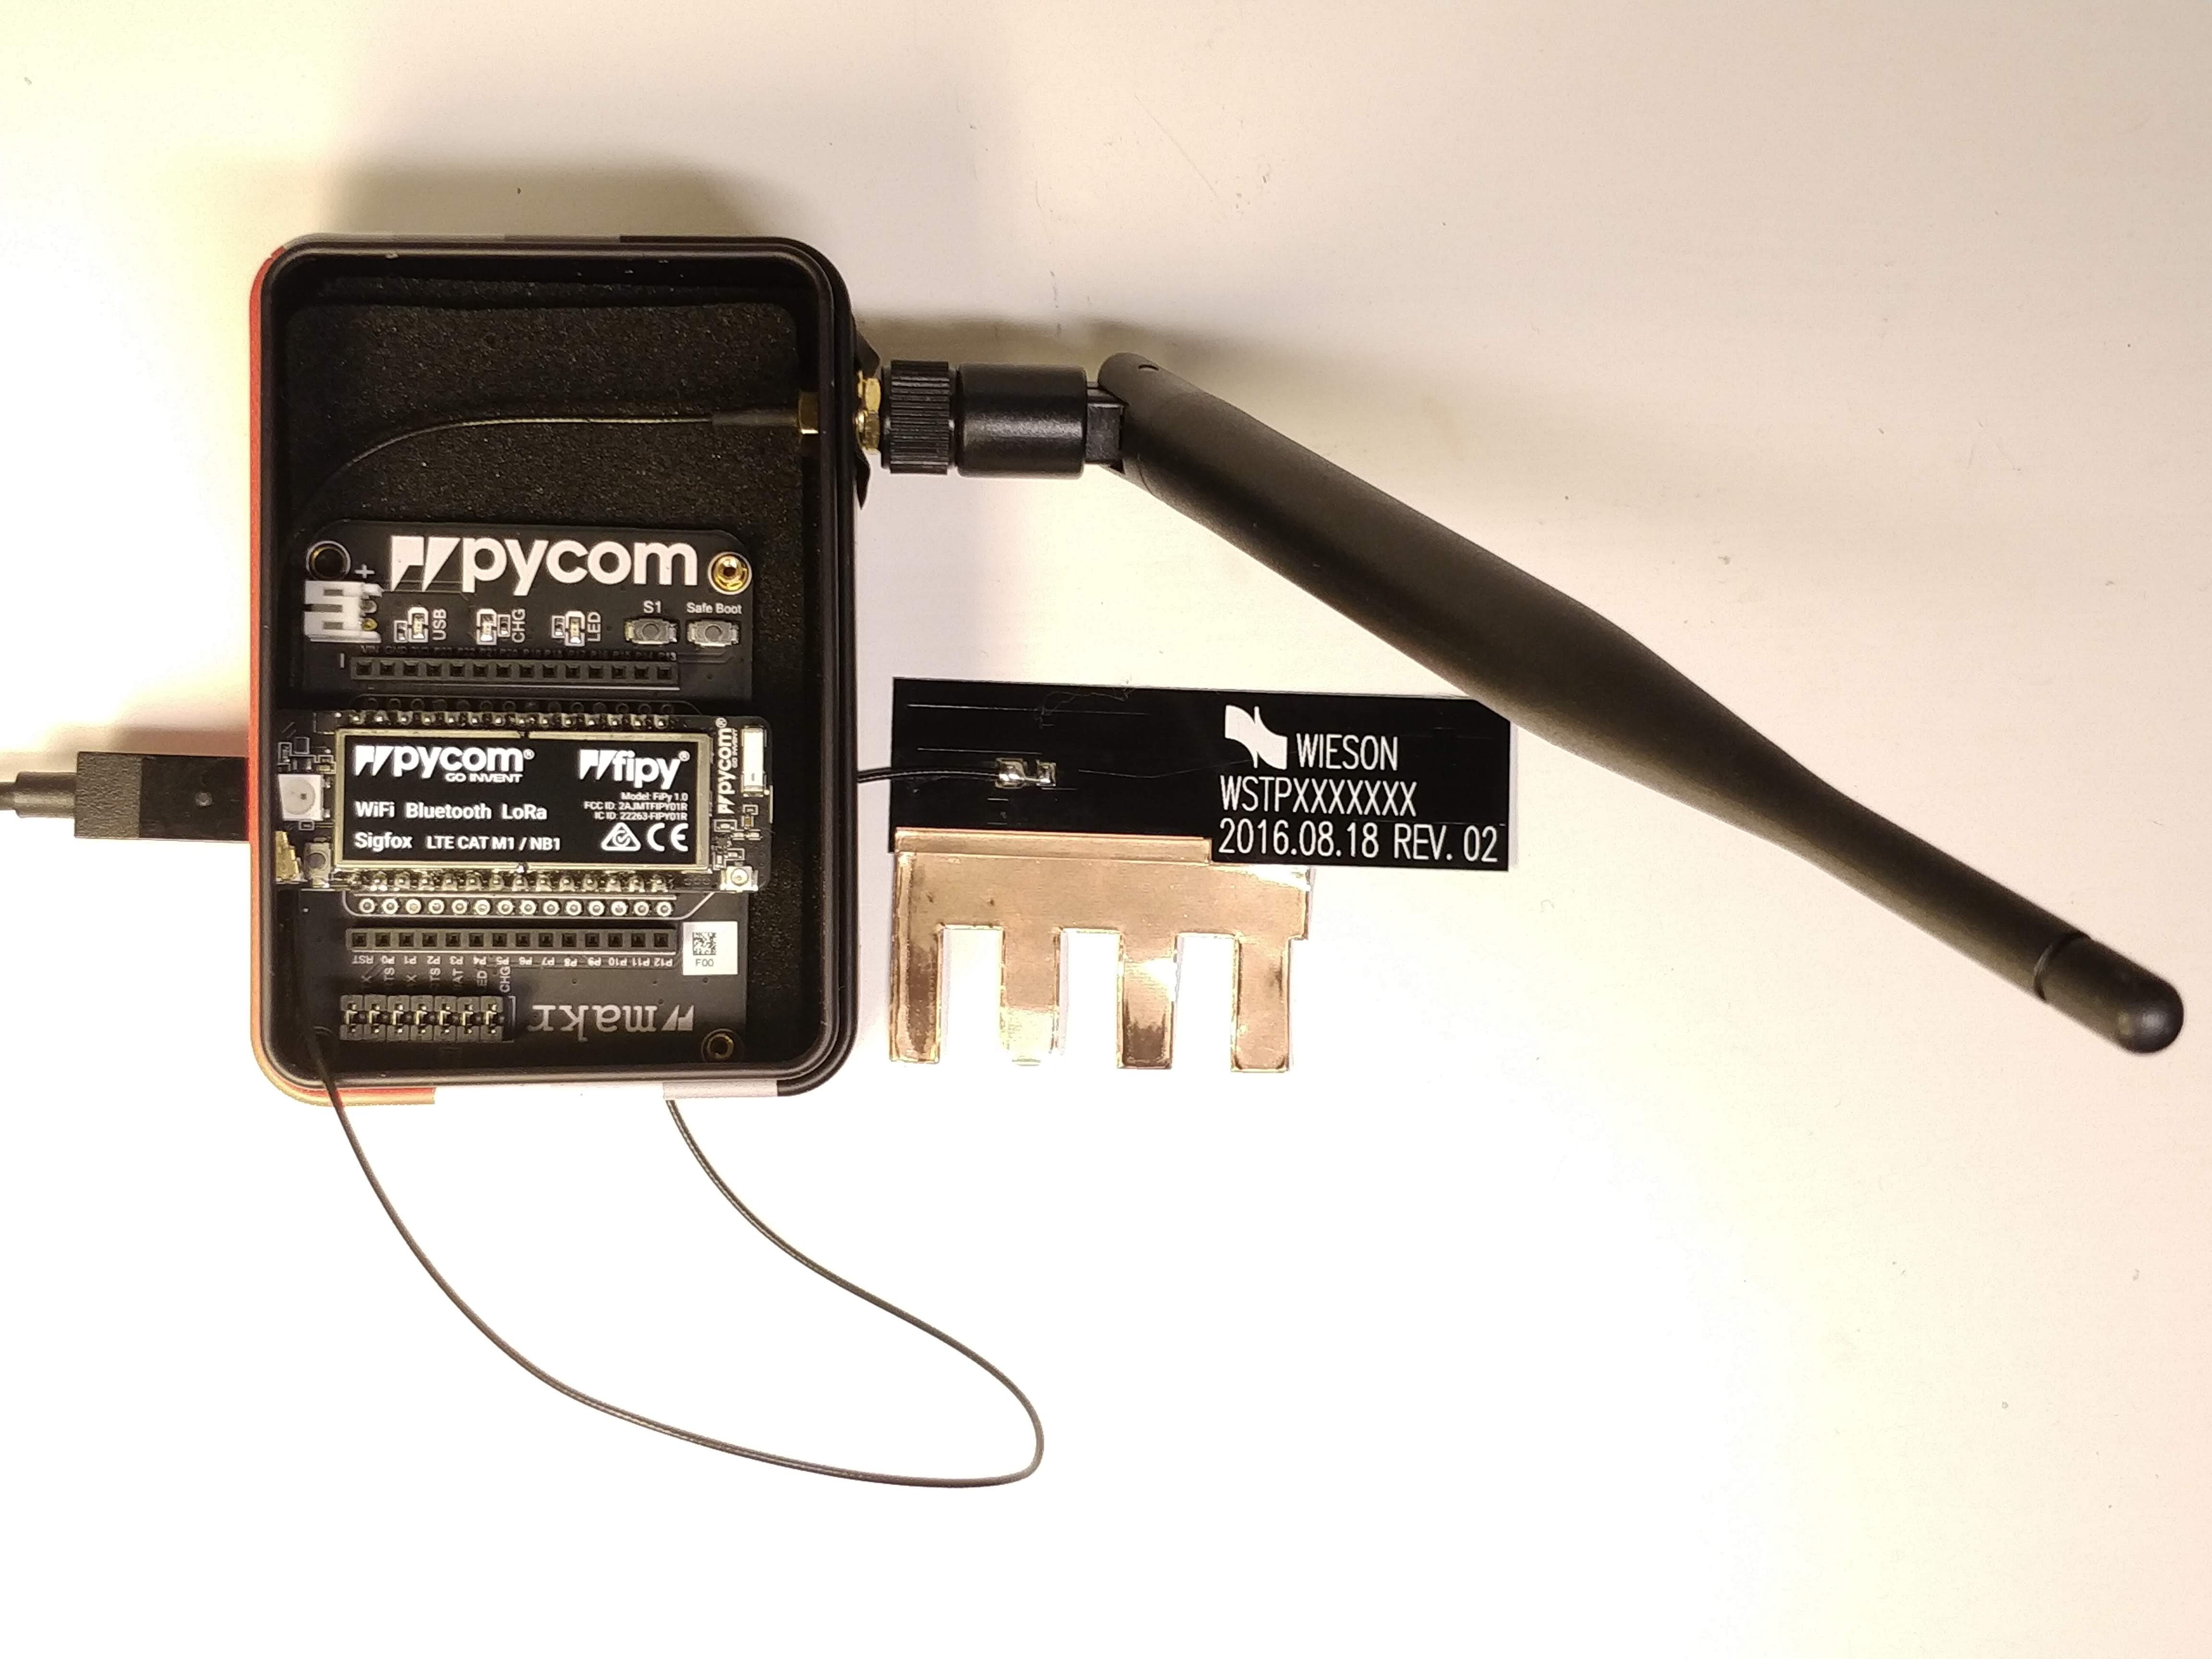
\includegraphics[width=0.8\textwidth]{figures/fipy.jpg}
            \caption{FiPy lõppseade mitme võrgu testimiseks.}
            \label{fig:fipy}
        \end{center}
    \end{figure}

    FiPy on katsetes lõppseadme rollis, ehk simuleerib üksikut IoT seadet suhtlemas iga uuritava LPWANi võrgu tugijaamadega.
    Lõppseadme vaatepunktist loob kirjeldatud kõik-ühes süsteem igati võrdsed tingimused katsete teostamiseks igale tehnoloogiale, arvestades järgmiseid asjaolusid:
    \begin{itemize}
        \item arendusplaat kasutab usaldusväärseid OEM modemeid,
        \item kõik modemid jagavad ühte mikrokontrollerit,
        \item arendusplaat ei ületa sätestatud signaalivõimsusi,
        \item antennid on seadmele kalibreeritud.
    \end{itemize}
% Katsete käigus kasutatakse lõppseadet, et luua side Sigfoxi, NORAneti, Telia NB-IoT ja isikliku LoRaWAN tugijaamaga strateegilistest kohtadest, mis on täpsemini kirjeldatud peatükis 4.3.
    Kasutatud testskript välja toodud lisades (Lisa 1).

    \subsection{LoRaWANi tugijaam}

    Juhul kui ükski valmisvõrk ei ole rakenduseks sobilik, on võimalik luua isiklik LoRaWANi võrk või leviala.
    Esimese eelduseks on rakendusserver, milleks võib olla avalik võrk, nagu TTN või isiklikult hostitud LoRaWAN serveri implementatsioon.
    Oma levialaks on vajalik tugijaam, mis on ühelt poolt LoRaWANi sagedustel pidevalt kuulav LoRa seade ning teiselt poolt paketiedastaja, mis suhtleb rakendusserveriga ning edastab kuuldud pakette.
    Sellise paketiedastaja lihtsaimal kujul ehitamiseks on vaja LoRa transsiivermoodulit ning Internetivõimekusega mikrokontrollerit või Raspberry Pi-d.
    Sõltuvalt valitud konfiguratsiooni populaarsusest on võrdlemisi lihtne oma riistvarale leida avalik koodirepositoorium, millega LoRaWANi spetsifikatsioonile vastav tugijaam üles seada.

    Töö raames kasutatav seade on WiFi toega ESP32 mikrokontrolleri põhine arendusplaat TTGO v1, millel on Semtechi SX1276 LoRa transsiiver.
    Tugijaam on lisaks varustatud lühikese isotroopilise LoRa antenniga ja displeiga ning on koos akutoitega ilmastikukindlas karbis, et seda oleks lihtne välioludes rakendada (joonis~\ref{fig:omatugijaam}).
    Mikrokontroller on programmeeritud avalikust repositooriumist laenatud koodiga, mis võimaldab tööajal kaudset konfigureerimist ja monitoorimist üle veebi.
    Rakendusserverina kasutab seade TTN avalikku võrku.

    \begin{figure} [htbp]
        \begin{tabular}{c c}
            \begin{minipage}{0.42\textwidth}
                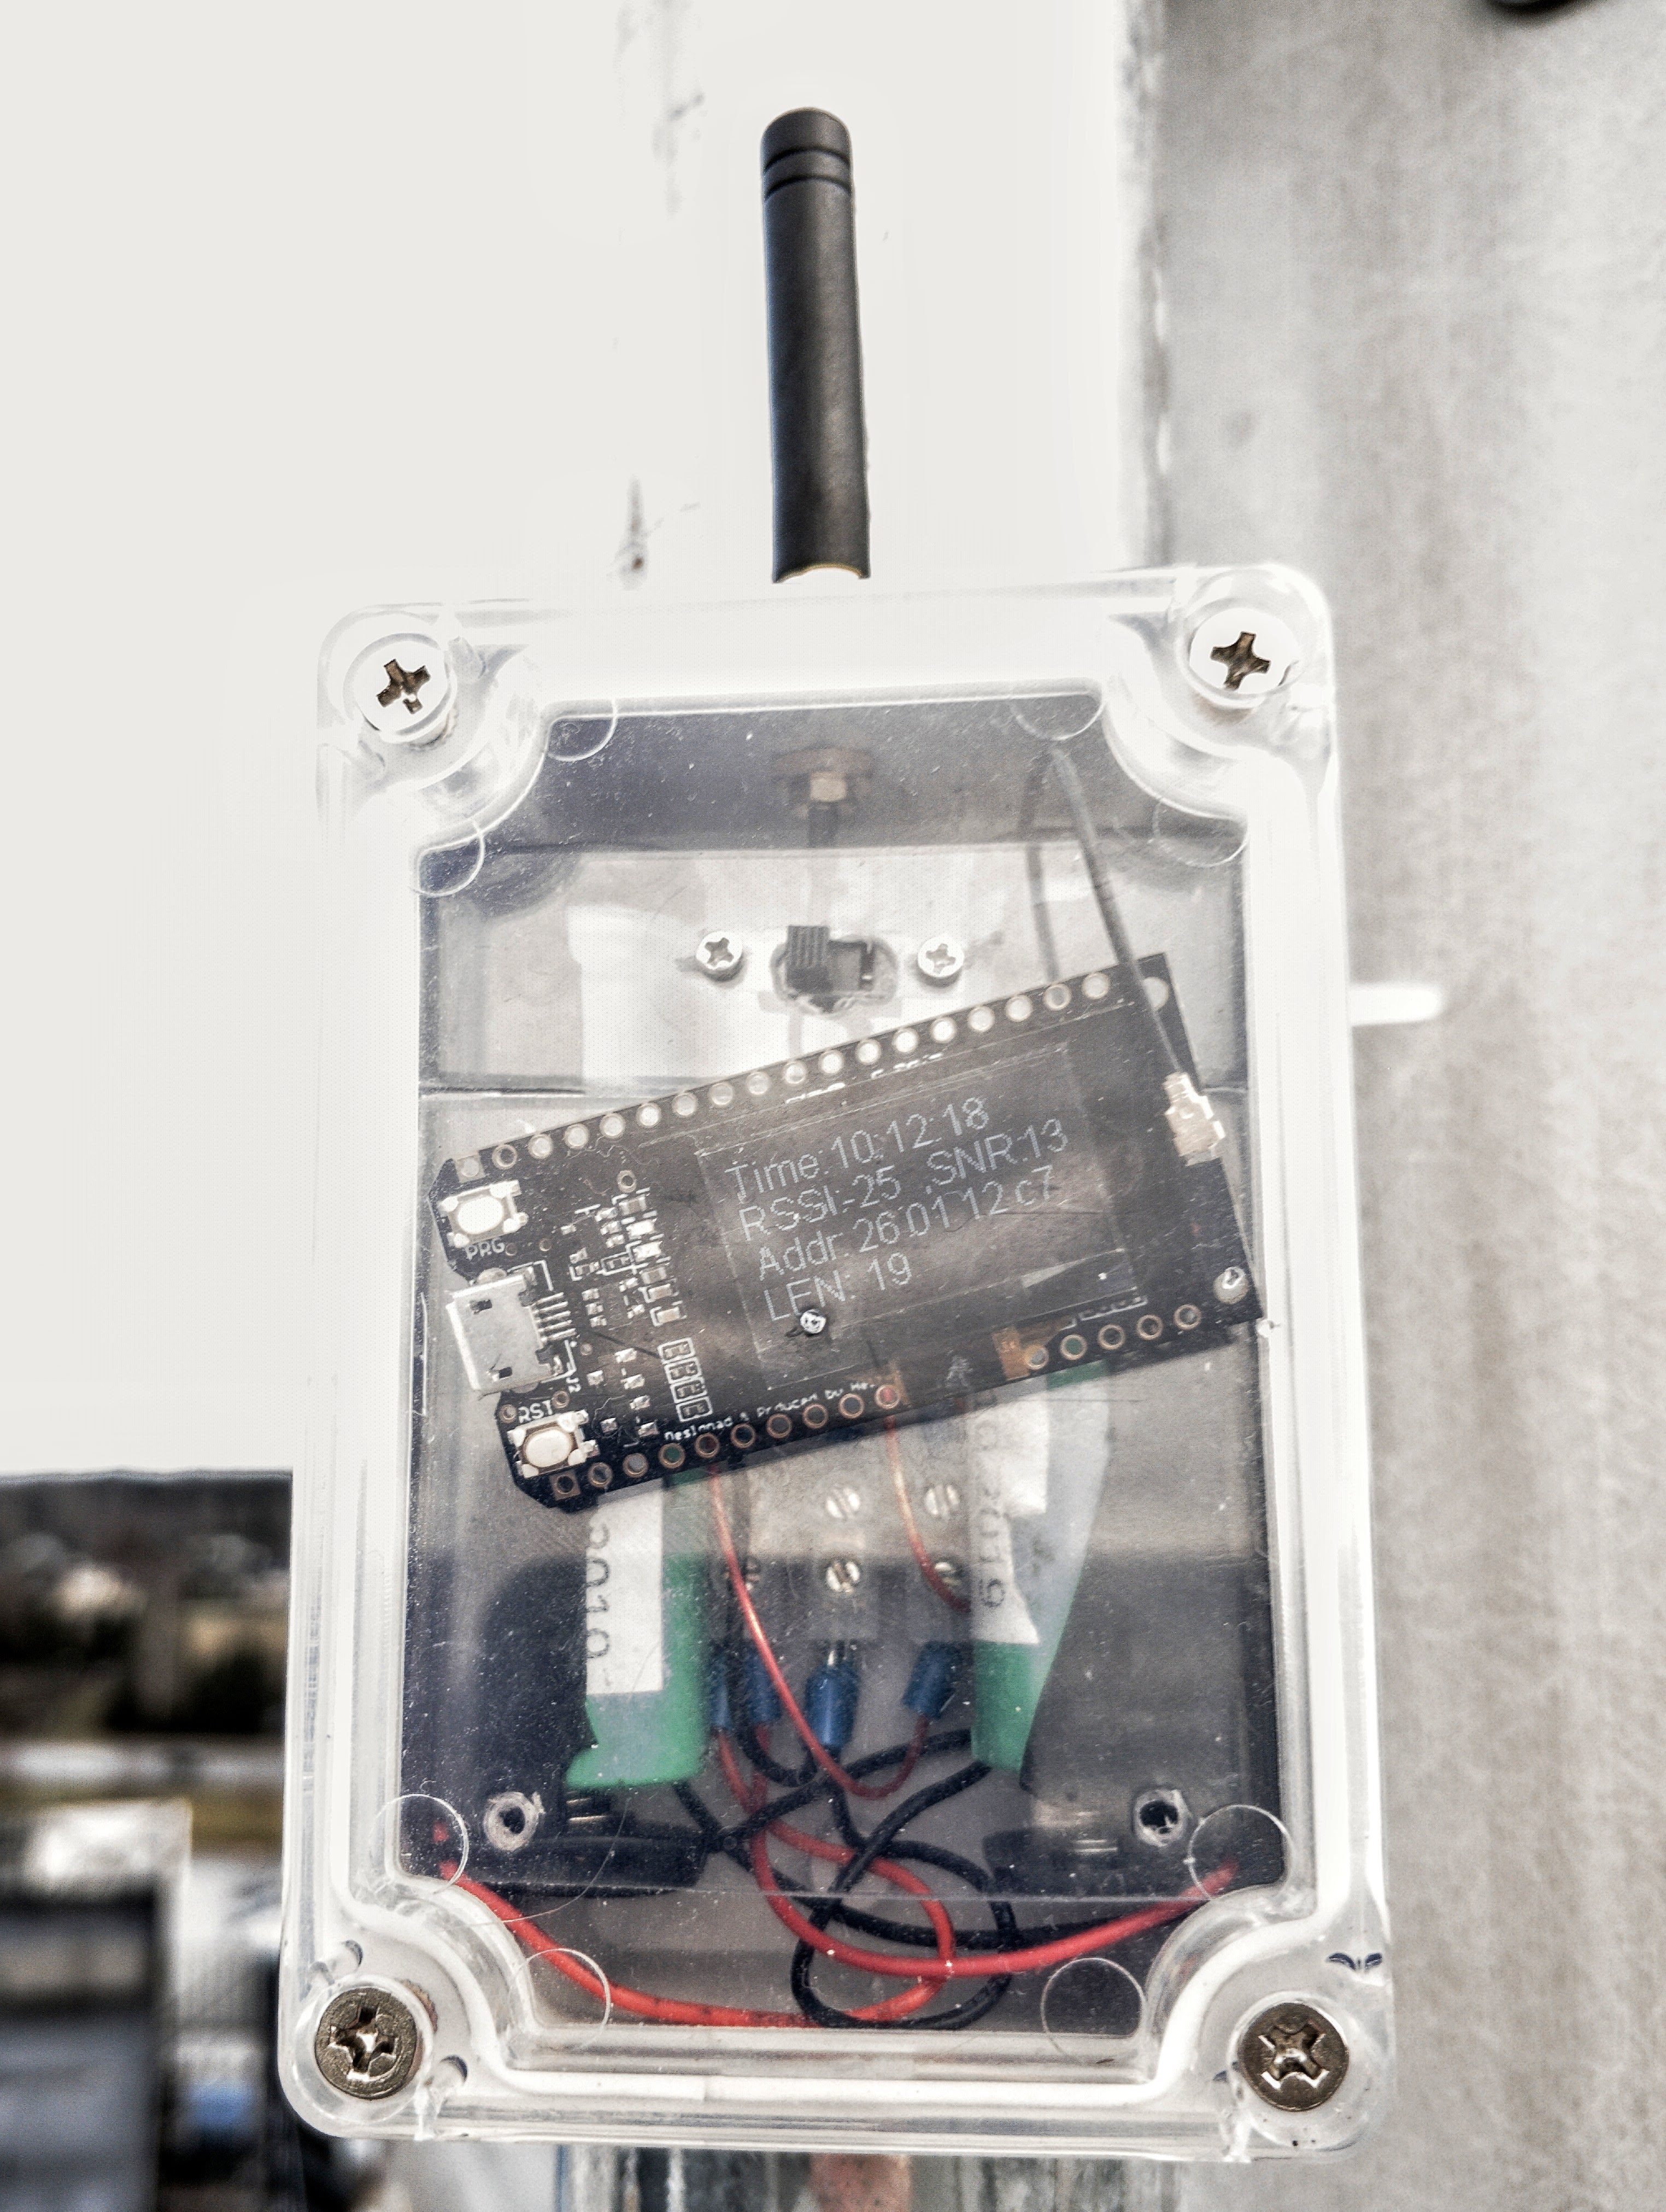
\includegraphics[width=\textwidth]{figures/ttn-jaam.jpeg}
            \end{minipage}
            &
            \begin{minipage}{0.53\textwidth}
                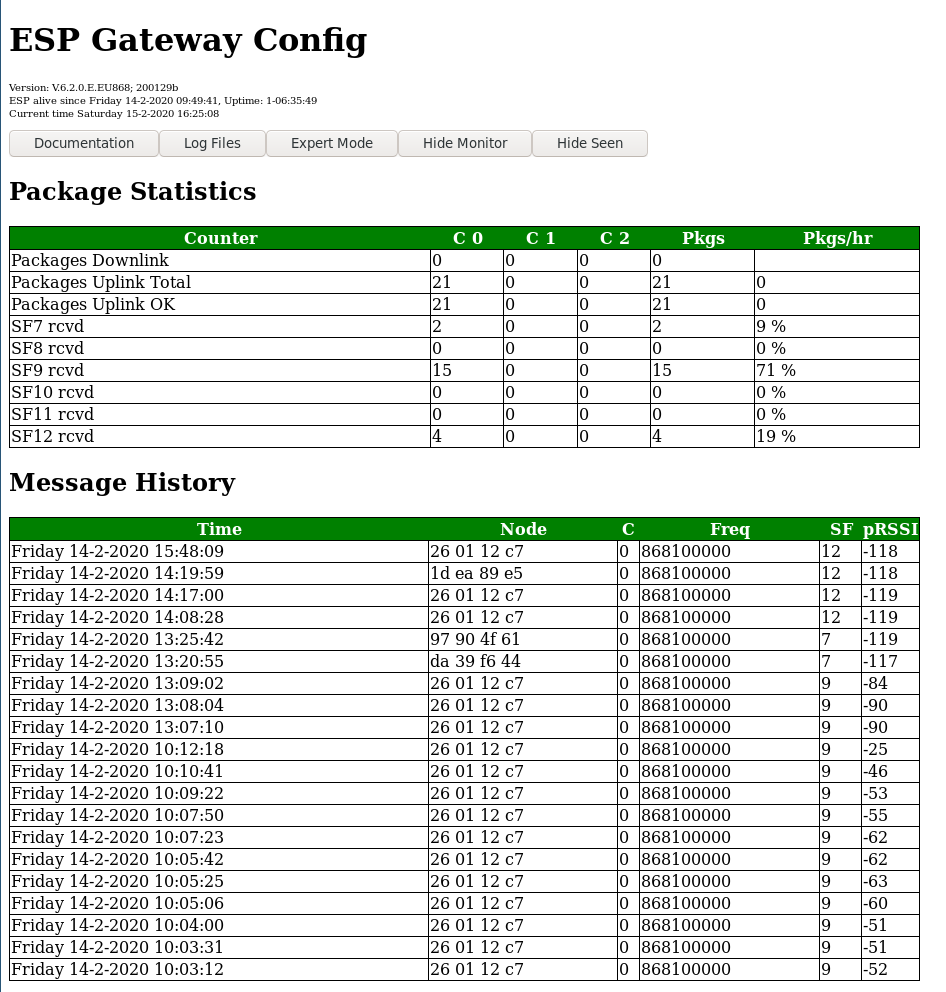
\includegraphics[width=\textwidth]{figures/ttn-jaama-liides.png}
            \end{minipage}
        \end{tabular}
        \caption{Isiklik LoRaWANi tugijaam ja selle veebiliides.}
        \label{fig:omatugijaam}
    \end{figure}

    Katsetugijaam on lihtsasti teisaldatav erinevatesse kohtadesse ning pääseb võrku läbi kaasasoleva WiFi pääsupunkti, mis on omakorda ühendatud LTE modemiga.
    Oluline on märkida, et tugijaam pole riistvarast tingitud piirangute tõttu täielikult LoRaWAN spetsifikatsioonile vastav ning on seetõttu sobiv vaid prototüüpimiseks.
    Erinevus täisväärtusliku tugijaamaga tuleneb transsiivermoodulist, mis on töökindel korraga teenindama vaid ühel kanalil ja laotusteguril.
    Sellise lahenduse mastaapne kasutamine võib liigselt koormata kitsast vahemikku 868 MHz sagedusest ning tekitada ebaproportsionaalselt häireid teiste sama piirkonna LoRa rakenduste töös.
    Erinevus kajastub ka hinnaklassis — täisvõimekusega LoRa modemi maksumus on 50-300€, käesoleva hind umbes 5€.

    \subsection{Katsete tingimused}

    Järgnevalt kirjeldatakse, millised on vaadeldavad tingimused, kus katseid läbi viiakse, ning mida on asukohtade valikul silmas peetud nii kasutusjuhte kui raskendavaid tegureid arvestades.
    Huvi pakkuvaid kriteeriume kontrollitakse kolmes keskkonnas, mis on omakorda käsitletud eraldi alapeatükkides: maapiirkond, linnapiirkond ja liikuv tugijaam.

    \subsubsection{Maapiirkond}

    Maapiirkonna all mõeldakse väiksema hoonestusega alasid, kus peamiseks side häirivateks faktoriteks on pinnamood ja mets.
    Asukoha valikul keskendutakse eelkõige keskkonna- ja põllumajandusrakenduste kriteeriumidele: levikaugus ja teenuse kvaliteet nii tugijaama silmsidega kui -sideta seadmetel.

    Vaadeldav piirkond on marsruudil Tartu-Elva-Otepää, mis pakub mitmekesist maastikku testideks nõgudes ja küngastel.
    Suurimateks väljakutseteks on levi ulatumine pinnavormide taha ja maksimaalne distants.
    Katseteks on LoRaWANi tugijaam kinnitatud Tartu Lõunakeskuse seitsmekorruselise hoone katusele.

    Kõrvalepõikena tehakse valik katseid lõppseadme liikumiselt maanteekiirusel, et kontrollida tehnoloogiate vastupanu Doppleri efektile, ehk lainesageduse moondumist vastuvõtja poole liikudes, mille olulisust eriti Sigfoxi ülikitsasriba modulatsioonile on välja toonud Kalfus ja Hégr~\cite{kalfus2016ultra}.

    \subsubsection{Linnapiirkond}

    Linnapiirkonna puhul peetakse silmas tihedat asustust.
    Kontrollitakse targa linna keskseid rakendusi, kus lõppseadmed asetsevad kohtades nagu korterid, keldrid või tänavad, varjatud hoonete ja muude takistustega.
    Olulisemad kriteeriumid, mis annavad tehnoloogiale eelise on läbistavus ja peegeldumine.

    Piirkond hõlmab peamiselt Tartu Annelinna ja kesklinna linnaosi.
    Side luuakse varieeruvates sügavustest kortermajade varjust, hoonete sisemustes ja keldrites.
    LoRaWANi tugijaam on nendeks katseteks asetatud Tartu Tasku keskuse Plasku hoone katusele.

    \subsubsection{Liikuv tugijaam}

    Eraldiseisvalt uuritakse veel andmete kogumist transporditavalt tugijaamalt.
    Testide puhul näeb see ette nii tugijaama kui lõppseadme asetsemist maapinna ligidal või hoones.
    Selliste stsenaariumidega jäljendatakse väiksema piirkonna sensoritelt info kogumist näiteks autos asetseva tugijaama abil.

    Katses rakendatakse loodud LoRaWANi tugijaama kahes asukohas: korteri tualettruumi valamukapis veearvestil ja kortermaja prügikonteinerite läheduses.
    Raskendavad asjaolud vastavalt asukohale on ekstreemne läbistavus ja levi maapinnalt maapinnale erinevate takistustega.

    \newpage


    \section{Tulemused}

    Katsete käigus on oluline meeles pidada erisusi teenuste teeninduspiirkondades.
    Erinevate meetodite abil on võimalik saada ettekujutus tugijaamade tegelikest asukohtadest, mis aitab edasisi mõõtmisi targemini tõlgendada.
    NB-IoT puhul aitas ühendatud sidemaste lokaliseerida \textit{Cellmapper}\footnote{https://www.cellmapper.net/map (22.03.2020)} keskkond, NORAnet veebiliides avaldab kätte saadud tugijaamade täpsed koordinaadid oma veebiliideses.
    Sigfoxi jaamade asukohad pole avalikult leitavad, kuid on umbkaudselt tuletatavad veebiliidesest kättesaadava levi kaardi abil.
    Joonisel~\ref{fig:tugijaamad} on kujutatud tugijaamad, millega saavutati ühendus üle kõikide katsete.

    \begin{figure} [ht]
        \begin{center}
            \includegraphics[width=0.95\textwidth]{figures/tugijaamad.png}
            \caption{Leitud tugijaamad.}
            \label{fig:tugijaamad}
        \end{center}
    \end{figure}

    Mastaapseimat kattuvust pakub Telia, mille infrastruktuur tugineb suuresti olemasolevatele LTE jaamadele, mis on seadistatud serveerima ka NB-IoTd.
    NORAnetil on kuus ning Sigfoxil viis tugijaama Tartu piirkonnas, mis on palju hõredam kui NB-IoTl.

    Maapiirkonnas tehti katseid 14 erinevast asukohast (joonis~\ref{fig:maapiirkonnakatsed}). Pelgalt ühenduse loomisega viieteistkümne kilomeetri raadiuses Tartu kesklinnast lõuna poole saavad eranditult hakkama NB-IoT ja Sigfox.
    Võttes arvesse NB-IoT jaamade hulka, on tagantjärele selge, et levialast välja sattumine on tugijaamade liiasuse ja teeninduspiirkondade kattuvuse tõttu väga keeruline.
    Selgemini saab võrrelda Sigfoxi ja NORAneti.
    Sügavamates nõgudes ja metsades esines NORAneti võrgus paketikadu ning mitmel korduskatsel oli näha, et side töötas oma võimekuse piiril, raporteerides -122 dBm vastuvõetud signaalitugevust ning SNR väärtusega -17 ehk raadiomüra tasemest 17-kordselt nõrgemat signaali.
    Sigfoxi puhul asetseb lävi palju kõrgemal -- kõige nõrgem saavutatud ülekanne antud raadiuses oli -132 dBm ning paketikadu ei täheldatud.

    Erinevalt kolmest teenusvõrgust, on oma tugijaama lahendusel vaid üks keskne pääsupunkt, mistõttu sai kontrollitumalt kombata levikauguse piire, ilma et seade mõne muu jaamaga haakuks.
    Silmsidega katsetel saavutati suurim distants 35 kilomeetri kaugusel asuvast Tehvandi suusahüppetornist ning ka nõlval, poole tee peal Pangodis.
    Samas vähegi reaalsemates oludes -- väiksemates metsatukkades, nõlvade varjus või majade vahel kadus side täielikult isegi seitsme kilomeetri raadiuses.

    Maanteekiirusel testides iga teenuse kindla leviala piires ei täheldatud liikumisest tingitud paketikadu.
    NB-IoT puhul avaldus probleem hoopis selle võimetusest haakida end implitsiitselt uue sidemasti külge, jõudes selle masti levialast välja, millega esmalt ühendati.
    Probleem väljendub enim selles, et haakimisprotseduur võttis üle kõikide katsete aega keskmiselt 20 sekundit, mis kergitab latentsi ning sellele eelnevalt puudub võimalus allalink sõnumiteks.

    Linnatänavatel oli paiku kokku seitse (joonis~\ref{fig:annelinn}).
    LoRa puhul võis ka Annelinna majade vahel leida leviauke nii NORAneti kui oma tugijaamaga, kusjuures oma tugijaam kaotas side juba vähimagi hoonestuse varjega pooleteise kilomeetriselt distantsilt.
    Sigfoxi jaoks oli Annelinn tugijaamadega varustatavust arvestades keerulistes tingimustes, kuid sellegipoolest ei tuvastatud välitingimustes paketikadu isegi kui ühes asukohas küündis vastuvõetud signaalitugevus -141 dBm-ni.
    NB-IoT välitingimustel probleeme ei tekitanud ning üleslink latents püsis pidevalt 0,3--0,5 sekundi vahemikus.

    \begin{figure} [p]
        \begin{center}
            \vspace*{-0.5cm}
            \includegraphics[width=1\textwidth]{figures/annelinn.png}
            \caption{Linnakatsete tulemused.}
            \label{fig:annelinn}
        \end{center}
    \end{figure}

    \begin{figure} [p]
        \begin{center}
            \vspace*{-0.5cm}
            \includegraphics[width=1\textwidth]{figures/maapiirkonnakatsed.png}
            \caption{Maapiirkonna katsete tulemused.}
            \label{fig:maapiirkonnakatsed}
        \end{center}
    \end{figure}

    Katseid siseruumides tehti neljas linnasiseses asukohas.
    Tartu Ülikooli Delta hoone keldrikorrusel kaotasid täielikult signaali Sigfox ja kumbki LoRaWAN teenus.
    Samas kohas oli NB-IoTl raskusi võrku ühendumise protseduuriga, ning õnnestumisel küündis 16 baidise COAP paketi latents 1,17 sekundini.
    Deltas said Sigfox ja NORAnet oma levi tagasi alates esimesest korrusest.
    Oma tugijaamaga kommunikeerida ei õnnestunud, isegi kui see asus Plasku hoone katusel koos NORAneti tugijaamaga, millega omakorda side saavutati.
    Viimane viitab tõenäoliselt antenni erinevustele, milles Levikomi seadmetel on eelis.
    Kahes katsealuses paneelmaja keldris töötas NB-IoT tõrgeteta ja alla sekundilise latentsiga, Sigfoxi läbistusvõime oli samuti väga hea.
    Kesklinna kortermaja keldris oli NORAnet ainuke, mis ühendust ei loonud.

    LoRaWANi ja oma tugijaama lühikesel distansil proovides katsetati läbistavust nii hoones sees kui ka vabas õhus maapinnalt.
    Joonisel~\ref{fig:lahikatsed} on kujutatud katseid kummagi tugijaama asetusega.
    Piki tänavat põhjapoole liikudes võimaldas veemõõtjat imiteeriv LoRa seade minna 415 meetri kaugusele, kuni esimese kurvini teel.
    Lõuna pool ehk kaugemast küljest oli distantsi võimalik suurendada vaid 100 meetrini, kuni ükski pakett isegi suurima laotusteguriga kohale ei jõudnud.
    Külgsuunas jõuti võimekuse piirini 350. meetril.
    Asetades seadme maja taha maapinnale, pikenes lõuna- ehk majataguses suunas distants 300 meetrini ning hoolimata vahetust takistusest kortermaja näol jäi põhjasuunal tulemus samaks.
    Külgsuunas, mis nüüd kannatas kannatas suurima varje ees ei levinud üle 200 meetri.

    \begin{figure} [ht]
        \begin{center}
            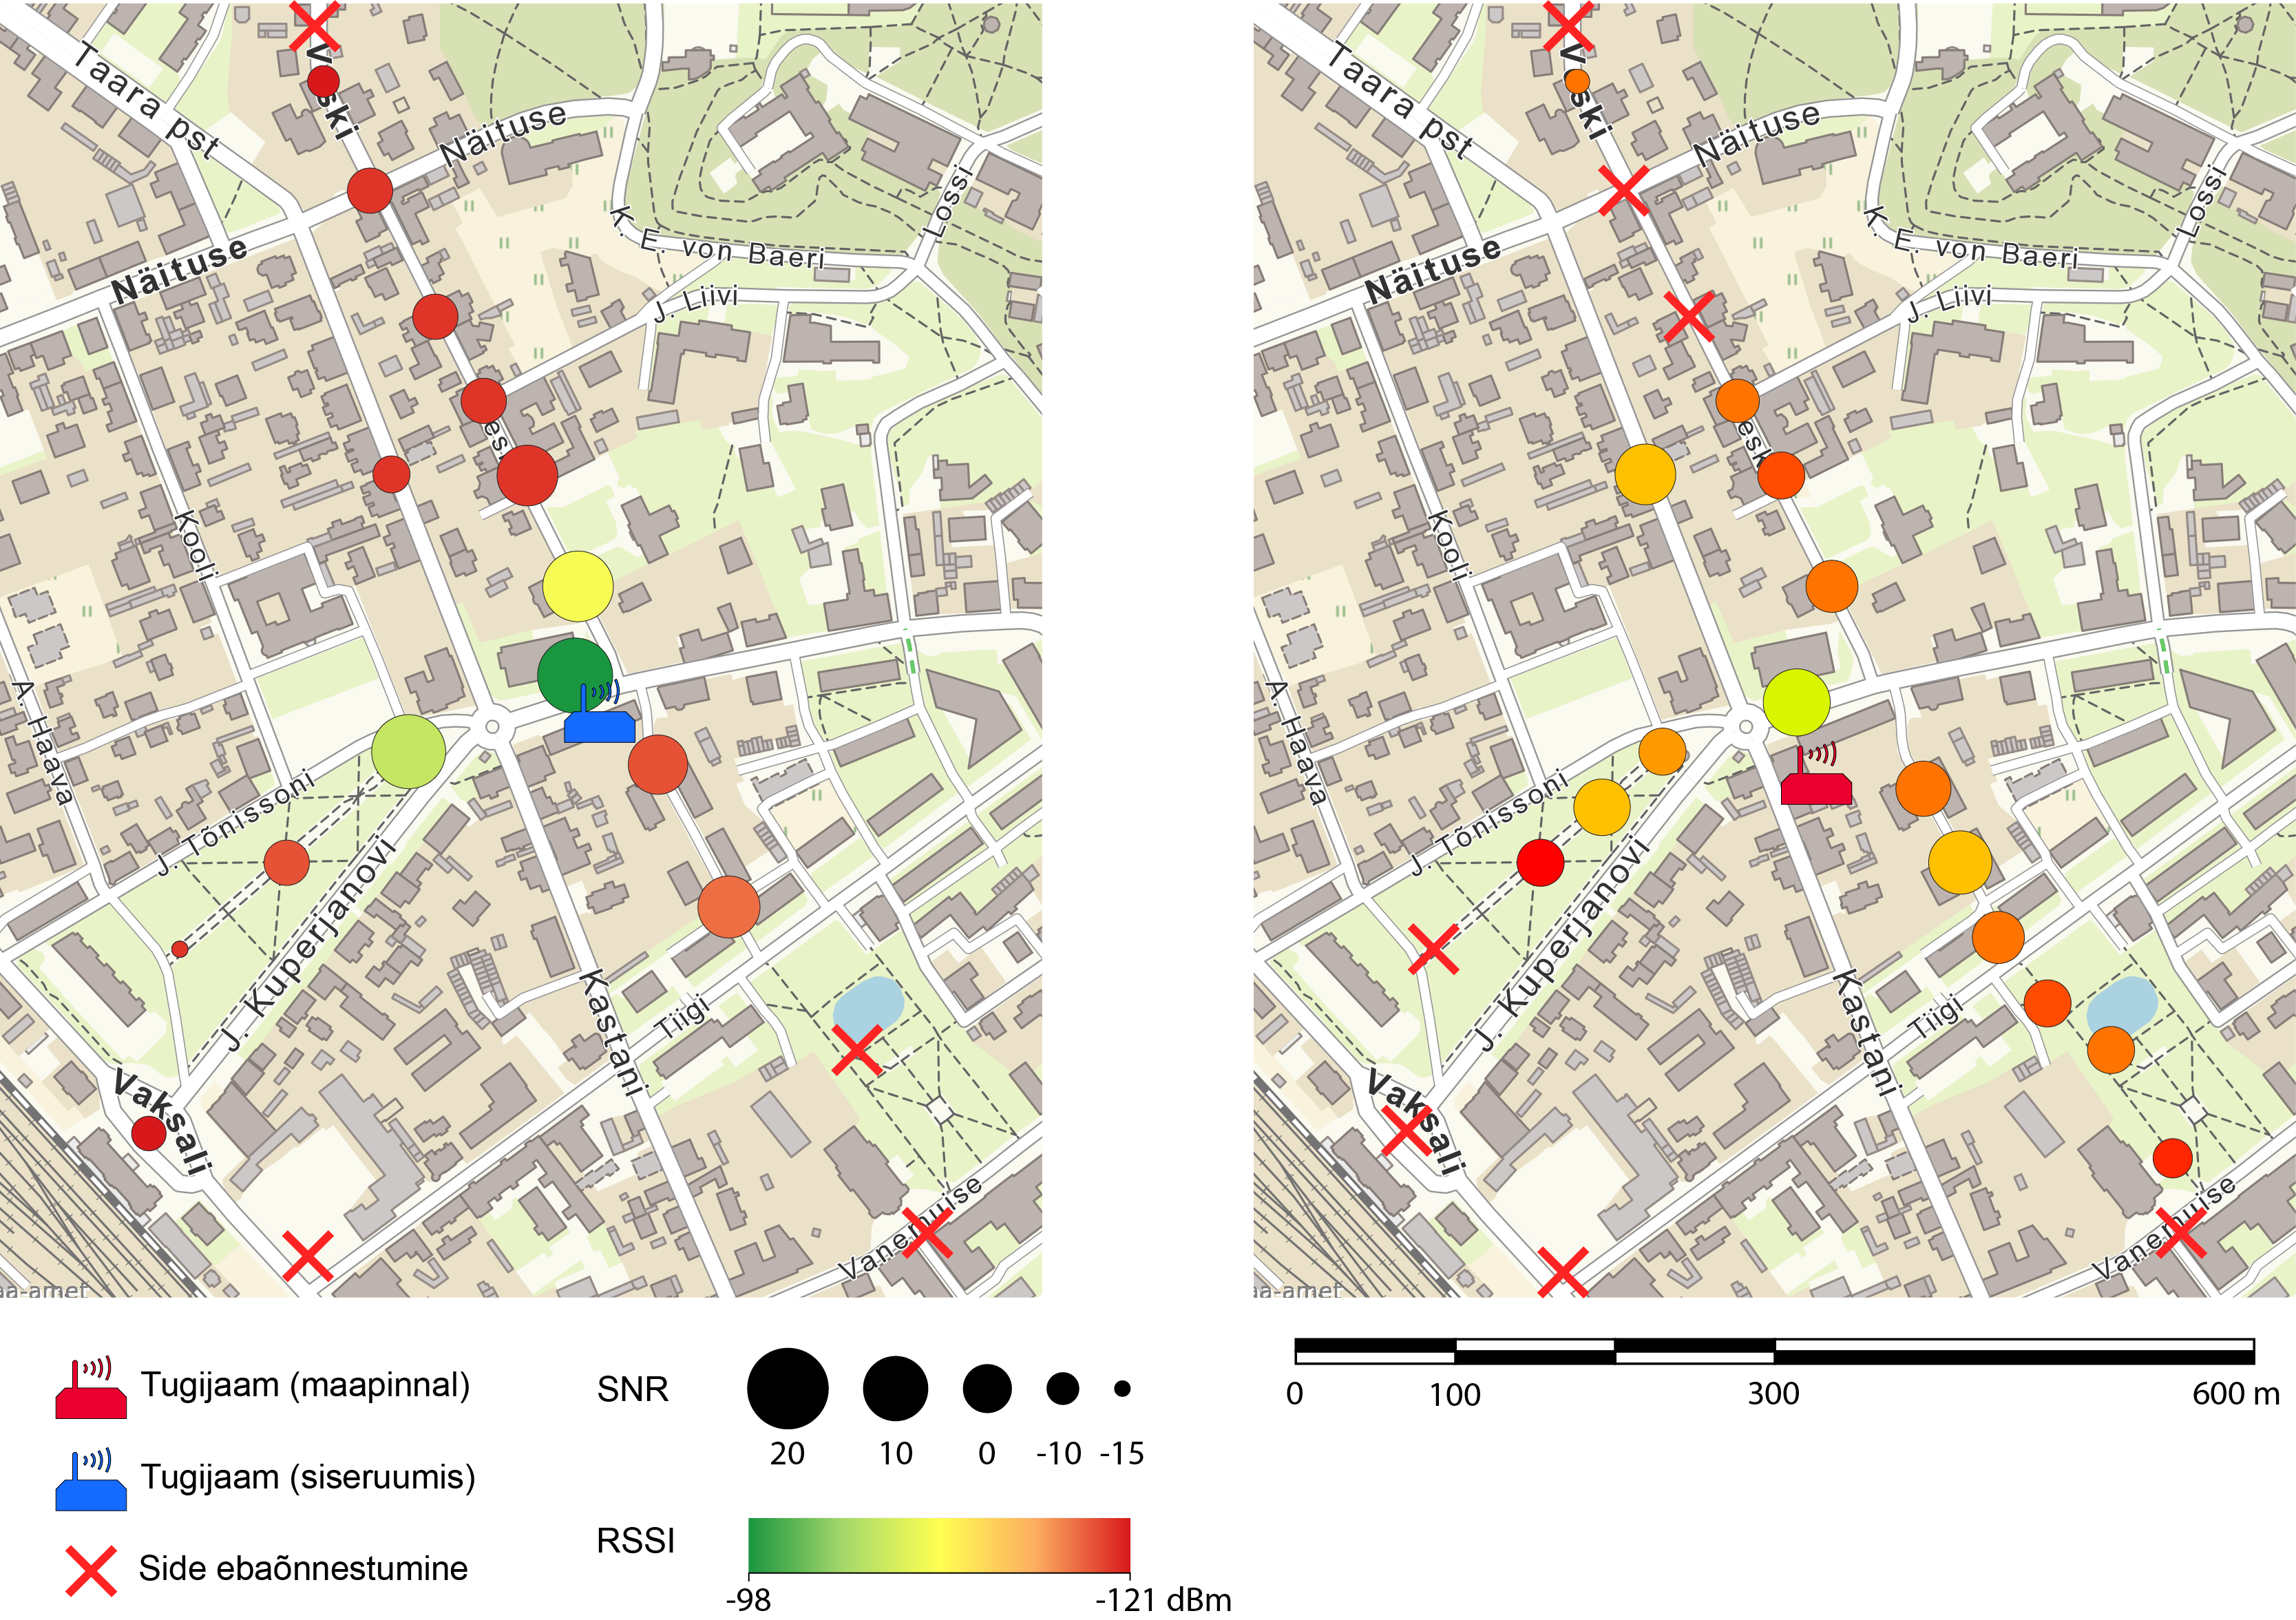
\includegraphics[width=0.95\textwidth]{figures/lahikatsed.png}
            \caption{Lähikatsete tulemused kahe tugijaama asetuse suhtes.}
            \label{fig:lahikatsed}
        \end{center}
    \end{figure}

    \newpage


    \section{Diskussioon}
    \TODO{Siia ilmub arutlus/analüüs, mis tehnoloogia on sobiv erinevatele kasutusjuhtudele, milline ei sobi üldse jne. Ühtlasi ilmutatakse siin vastus uurimisküsimusele}
    \newpage


    \section{Kokkuvõte}

    \newpage

% BibTeX bibliography
    \bibliographystyle{unsrt} %plain=[1], alpha=[BGZ09]
    \bibliography{../src/bachelor-thesis}
    \TODO{Viidete formaat. Osad viited veel käsitsi pandud, mistõttu on numbrid valed}

    \addcontentsline{toc}{section}{\refname}


% Use Biblatex if you have problems with Estonian keywords
%\printbibliography %biblatex


    \newpage
    \appendix
%\section*{\appendixname}
    \section*{Lisad}
    \addcontentsline{toc}{section}{Lisad}


    \section*{I. Testskriptid}
    \addcontentsline{toc}{subsection}{I. Lõppseadme testskriptid}

    \newpage

%=== Licence in Estonian
    \newcommand\EstLicence{{%
        \section*{II. Litsents}

        \addcontentsline{toc}{subsection}{II. Litsents}

        \subsection*{Lihtlitsents lõputöö reprodutseerimiseks ja üldsusele kättesaadavaks tegemiseks}

        Mina, \textbf{Kert Tali},

        \begin{enumerate}
            \item
            annan Tartu Ülikoolile tasuta loa (lihtlitsentsi) minu loodud teose
            \par
            \textbf{LPWAN raadiovõrkude võrdlus ja kasutusjuhud Tartu näitel},
            \par
            mille juhendaja on Alo Peets,
            \par
            reprodutseerimiseks eesmärgiga seda säilitada, sealhulgas lisada digitaalarhiivi DSpace kuni autoriõiguse kehtivuse lõppemiseni.
            \par
            \item
            Annan Tartu Ülikoolile loa teha punktis 1 nimetatud teos üldsusele kättesaadavaks Tartu Ülikooli veebikeskkonna, sealhulgas digitaalarhiivi DSpace kaudu Creative Commonsi litsentsiga CC BY NC ND 3.0, mis lubab autorile viidates teost reprodutseerida, levitada ja üldsusele suunata ning keelab luua tuletatud teost ja kasutada teost ärieesmärgil, kuni autoriõiguse kehtivuse lõppemiseni.
            \item
            Olen teadlik, et punktides 1 ja 2 nimetatud õigused jäävad alles ka autorile.
            \item
            Kinnitan, et lihtlitsentsi andmisega ei riku ma teiste isikute intellektuaalomandi ega isikuandmete kaitse õigusaktidest tulenevaid õigusi.
        \end{enumerate}

        \noindent
        Kert Tali\\ %author's name
        \textbf{\textsl{pp.kk.aaaa}}
    }}%\newcommand\EstLicence


    \EstLicence


\end{document}

